\documentclass[a4paper,12pt,Times]{article}
\usepackage{abakos}  %pacote com padrão da Abakos baseado no padrão da PUC

%%%%%%%%%%%%%%%%%%%%%%%%%%%
%Capa da revista
%%%%%%%%%%%%%%%%%%%%%%%%%%
%\setcounter{page}{80} %iniciar contador de pagina de valor especificado
\newcommand{\monog}{Trabalho Prático (Parte I)}
\newcommand{\monogES}{Model - Pratical Exercise - ICEI - Puc Minas}
\newcommand{\tipo}{Artigo }  % Especificar a seção tipo do trabalho: Artigo, Resumo, Tese, Dociê etc
\newcommand{\origem}{Brasil}
\newcommand{\editorial}{\textbf{Puc Minas}, Belo Horizonte, Set. 2021}  % p. xx-xx – páginas inicial-final do artigo
% \newcommand{\lcc}{\scriptsize{Licença Creative Commons Attribution-NonCommercial-NoDerivs 3.0 Unported}}

%%%%%%%%%%%%%%%%%INFORMAÇÕES SOBRE AUTOR PRINCIPAL %%%%%%%%%%%%%%%%%%%%%%%%%%%%%%%
\newcommand{\AutorA}{Matheus Rangel Figueiredo}
\newcommand{\AutorB}{Diogo Fasciani Viggiani Rios de Castro}
\newcommand{\funcaoA}{}
\newcommand{\emailA}{matheus.figueiredo.1275135@sga.pucminas.br}
\newcommand{\emailA}{matheus.figueiredo.1275135@sga.pucminas.br}
\newcommand{\emailB}{dfvrcastro@sga.pucminas.br}
\newcommand{\cursA}{Ciência da Computação PUC Minas}
\newcommand{\cursB}{Ciência da Computação PUC Minas}


% Definir macros para o nome da Instituição, da Faculdade, etc.
\newcommand{\univ}{PUC Minas}

\newcommand{\keyword}[1]{\textsf{#1}}

\begin{document}
% %%%%%%%%%%%%%%%%%%%%%%%%%%%%%%%%%%
% %% Pagina de titulo
% %%%%%%%%%%%%%%%%%%%%%%%%%%%%%%%%%%

\begin{flushleft}

\begin{minipage} [c][5cm][b]{16.5cm} % a primeira minipágina tem uma altura de 1.5cm e uma largura de 2.3cm.
% comando que introduz o logo da escola que nesta altura já terá de estar na pasta imagens que 
%por sua vez está na pasta onde se guardou o arquivo tex. E introduzimos essa imagem com a mesma altura da minipage.

\includegraphics[scale=1.1]{figuras/pucmg.png} 
\end{minipage}

 \vspace{0cm} {
 \singlespacing \Large{\monog \symbolfootnote[1]{Artigo apresentado à Revista Abakos} \\ }
  \normalsize{\monogES}
 }
\end{flushleft}
\begin{flushright}
\singlespacing 
\normalsize{\AutorA \footnote{\funcaoA \cursA, \origem -- \emailA }} \\
\normalsize{\AutorB \footnote{\funcaoB \cursB, \origem -- \emailB }} \\


\end{flushright}
\thispagestyle{empty}

\begin{abstract}
\noindent
Este exercício prático contem a documentação do trabalho prático I (Parte I), feita em \LaTeX. O programa é um sistema de cadastro de prontuários para uma empresa de planos de saúde. O menu de opções do programa é composto de 6 alternativas (sendo uma delas a opção de sair do programa), é possível: 1- criar um arquivo, 2- inserir registros, 3- editar registros, 4- remover registros, 5- imprimir os registros e 0- sair do programa. Todo o projeto foi desenvolvido na linguagem de programação java e tem autoria do grupo conforme exigido na documentação. O intuito do programa é facilitar o cadastro dos pacientes no sistema, é possível consultar toda a lista de pacientes cadastrados, cadastrar novos pacientes e fazer a exclusão dos mesmos, também é possível olhar informações inseridas no prontuário como nome (máximo de 20 bytes + 2 para o tamanho da string), sexo, cpf (máximo de 9 bytes + 2 para o tamanho da string), data de aniversário e as anotações medicas feitas para cada paciente.
\\\textbf{\keyword{Palavras-chave: }}\LaTeX. Exercício Prático. Java.
\end{abstract}

%%%%%%%%%%%%%%%%%%%%%%%%%%%%%%%%%%%%%%%%%%%%%%%%%%%%%%%%%
\newpage 


\selectlanguage{brazilian}
 \onehalfspace  % espaçamento 1.5 entre linhas
 \setlength{\parindent}{1.25cm}

%%%%%%%%%%%%%%%%%%%%%%%%%%%%%%%%%%%%%%%%%%%%%%%%%
%% INICIO DO TEXTO
%%%%%%%%%%%%%%%%%%%%%%%%%%%%%%%%%%%%%%%%%%%%%%%%%

\section{\esp Menu}
O programa é compilado no Main.java. Ao rodar o programa será apresentado ao usuário um menu que é a tela principal do programa
\\
\begin{figure}[ht]
	\centering	
	
	\vspace{-0.4cm}
	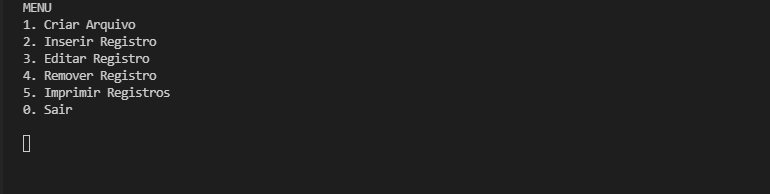
\includegraphics[width=1.0\textwidth]{figuras/imagem_2021-09-01_170747.png}
	 \vspace{-0.2cm}
	\\\textbf{\footnotesize Fonte: Visual Studio Code Screen Capture}
	\label{fig:figura1}
\end{figure}
\vspace{-0.5cm}

O menu é composto de 5 opções, e a opção '0' para sair do programa assim totalizando 6 opções:\\
             1- Criar um arquivo\\
             2- Inserir registros\\
             3- Editar registros\\
             4- Remover registros\\
             5- Imprimir os registros\\
             0- Sair do programa

\subsection{\esp Criar Arquivo}

Caso o arquivo não exista, será criado um arquivo com o nome pre definido de 'arq.db' e será perguntado ao usuário o tamanho máximo das anotações do médico. Então o arquivo será criado com um registro (tipo INT) já escrito que representa o tamanho máximo das anotações do médico. Entretanto se o arquivo já existir sera mostrado na tela uma mensagem informando que o mesmo já foi criado.

\subsection{\esp Inserir Registro}

Verifica se o arquivo já existe, se existir faz um formulário ao usuário perguntando sobre os atributos da classe Pessoa (com exceção do 'ativo' e das anotações do médico) e armazena esses dados em um objeto do tipo Pessoa. Então faz uma busca no arquivo procurando por lápides (ativo = false). A função irá inserir o objeto criado como um registro no local da primeira lápide encontrada. Caso não encontre lápides, o objeto sera registrado no final do arquivo. Após esses processos ira atualizar o cabeçalho aumentando em uma unidade o número de registros no arquivo.

\subsection{\esp Editar Registro}
 
Verifica se o arquivo já existe, se sim, pergunta o 'cpf' do registro que terá uma alteração nas anotações do médico. Então faz uma busca pelo 'cpf' inserido, caso não encontrado, emite uma mensagem informado que o 'cpf' não pode ser encontrado. Entretanto, caso encontrado, pergunta ao usuário qual será a nova anotação e a coloca no lugar da antiga.
 
 \subsection{\esp Remover registro}
 
 
 Verifica se o arquivo já existe, se sim, pergunta o 'cpf' do registro que será apagado. Então faz uma busca pelo 'cpf' inserido caso não encontrado, emite uma mensagem informado que o 'cpf' não pode ser encontrado. Entretanto, caso encontrado, altera o atributo 'ativo' do registro para 'false', indicando que o registro tornou-se uma lápide. Após esses processos ira atualizar o cabeçalho diminuindo em uma unidade o número de registros no arquivo.
 
 
 
 \subsection{\esp Imprimir registro}

Percorre todos os registros do arquivo e imprime aqueles que não são lápides (ativo = true).


\section{\esp Classe Pessoa}

Classe do programa que irá armazenar os atributos dos registros.
Registros: Atributo ativo do tipo booleano, se ele for 'true' quer dizer que o registro existe, caso contrario o mesmo é uma lapide.

\subsection{\esp Ativo}


Atributo ativo do tipo booleano. Se ele for 'true' quer dizer que o registro existe, caso contrario o mesmo é uma lapide (1 bayte é o tamanho do atributo ativo).

\subsection{\esp Cpf}

Atributo do tipo string que tem seu tamanho máximo limitado a 9 bytes. (9 bytes + 2 para o tamanho da string).



\subsection{\esp Nome}

Atributo do tipo string que tem seu tamanho máximo limitado a 20 bytes. (20 bytes + 2para o tamanho da string).


 \subsection{\esp Sexo}

Atributo do tipo char que pode ser 'm' ou 'f' (masculino/feminino), tem seu tamanho máximo limitado a 2 bytes.



\subsection{\esp Data de nascimento}

É separada em 3 atributos:\\
dia: Atributo do tipo byte\\
mês: Atributo do tipo byte\\
ano: Atributo do tipo short
   

\subsection{\esp Anotacoes}

Atributo especial da Classe Pessoa.
Atributo do tipo string de tamanho variável. O tamanho máximo da string será decidido na criação do arquivo.
   
\section{\esp Metadados}


O programa criará um arquivo para armazenar os registros. Esse arquivo tera o nome pre-definido como "arq.db". O programa ira separa o arquivo em 2 partes, o cabeçalho e os registros.


\subsection{\esp Cabeçalho}

O cabeçalho é o primeiro dado no arquivo. Nele serão armazenados os metadados. O tamanho do cabeçalho é de exatamente 8 bytes (2 inteiros). É composto por dois dados: tamanho das anotações e número de registros.

\subsubsection{\esp Tamanho das anotações}

É o primeiro metadado do arquivo, é representado por um numero inteiro (4 bytes). Esse dado delimita o número máximo de bytes possível nas anotações do medico de cada registro.


\subsubsection{\esp Número de registros}

É o segundo e último metadado do arquivo, é representado por um número inteiro (4 bytes). Esse dado representa o número de registros ativos (ativo = true) do arquivo.

\subsection{\esp Registros}

Os registros representam as pessoas cadastradas no sistema. Eles apresentam todos os dados de uma pessoa (representada pela Classe Pessoa).
O tamanho de cada registro é de 38 bytes + o tamanho máximo da string de anotações médicas (será declarado na criação do arquivo).


%%%%%%%%%%%%%%%%%%%%%%%%%%%%%%%%%%%
%% FIM DO TEXTO
%%%%%%%%%%%%%%%%%%%%%%%%%%%%%%%%%%%

% \selectlanguage{brazil}
%%%%%%%%%%%%%%%%%%%%%%%%%%%%%%%%%%%
%% Inicio bibliografia
%%%%%%%%%%%%%%%%%%%%%%%%%%%%%%%%%%%

 \newpage
 \singlespace{
 \bibliographystyle{abntex2-alf}
 \bibliography{bibliografia}
 \bibliographystyle{econ}
\bibliography{Reference1}
 }

\end{document}